\section{Introduction}
\label{sec:introduction}

In the realms of data management and analytics, relational databases have long been the bedrock of structured data storage and retrieval, empowering a plethora of applications,% across domains ranging from finance to healthcare and beyond.
The ubiquity of these databases has been supported by the advent of Structured Query Language (SQL)~\cite{chamberlin1974sequel}, a standardized language that has been adopted widely by various relational database management systems for managing data through schema-based operations. %SQL has been pivotal in the progression of data management, enabling the efficient manipulation of complex data structures and fostering interoperability between disparate systems.

Despite its considerable success and broad adoption, SQL has its limitations, particularly when it comes to representing and querying intricately linked data. Consider, for instance, the relational tables of \kk{Person} and \kk{Knows}, the latter symbolizing a many-to-many relationship between instances of the former. Constructing a SQL query to retrieve a group of four persons who are all mutually acquainted is not a straightforward endeavor, potentially leading to a cumbersome and complex SQL expression.

In comparison, such a scenario could be succinctly addressed using graph query languages, exemplified by Cypher~\cite{opencypher}, a language where queries are expressed as intuitive and concise graph pattern matching. This discrepancy between the relational and graph querying paradigms has given rise to the innovative SQL/Property Graph Queries (SQL/PGQ), an extension \revisewy{formally adopted in the ISO/IEC SQL:2023 standard}~\cite{sql-pgq}. SQL/PGQ is designed to amalgamate the extensive capabilities of SQL with the inherent benefits of graph pattern matching. With SQL/PGQ, it is now possible to define and query graphs within SQL expressions, transforming otherwise complex relational queries -- characterized by multiple joins -- into simpler and more intuitive graph queries.

\begin{example}
    \label{ex:introduction:sqlpgq}
    Consider the four relational tables in the database: \kk{Person(id, name, place\_id)}, \kk{Message(id, content, date)}, \kk{Like(p\_id, m\_id, date)}, and \kk{Place(id, name)}. Using SQL/PGQ, a property graph $G$ is articulated as a \lstinline{GRAPH_TABLE}, established on the basis of the first three tables. In this mapping, rows from \kw{Person} and \kw{Message} are interpreted as vertices with labels ``Person'' and ``Message'' respectively, while rows from Like represent edges with the label ``Likes''. This mapping process will be formally elaborated in \refdef{rgmapping}. An SQL/PGQ query to discover the friends of a person named ``Tom'' and the place they live in, where ``Tom'' and friends share an affinity for the same message, can be formulated as:
    \begin{lstlisting}
        SELECT p2_name, place.name
        FROM GRAPH_TABLE (G
            MATCH (p1:Person)-[:Likes]->(m:Message),
                  (p2:Person)-[:Likes]->(m:Message),
                  (p1)-[:Knows]->(p2)
            COLUMNS (
                p1.name AS p1_name,
                p1.place_id AS p1_place_id,
                p2.name AS p2_name)
        ) g JOIN Place place
            ON g.p1_place_id = place.id
        WHERE g.p1_name = 'Tom';
    \end{lstlisting}
    In graph $G$, a graph pattern matching is employed to decode the intricate relationships between persons and messages. Upon executing the pattern matching, a \lstinline{COLUMNS} clause projects the results into a tabular format, enumerating essential attributes. This resultant table is then joined with the \kk{Place} table to obtain the place's name.
\end{example}

The SQL/PGQ standard, while a significant leap forward in the realm of relational databases, primarily addresses language constructs. A discernible gap exists in the theoretical landscape, particularly in analyzing, transforming, and optimizing SQL/PGQ queries with hybrid relational and graph semantics. %This gap is mainly due to the absence of a unified framework for optimizing such hybrid queries, a framework that could bridge the divide between the well-established relational optimization techniques and the evolving domain of graph query optimization.

Relational query optimization has historically leaned on the \spj (selection-projection-join) skeleton~\cite{spj,Chaudhuri98}, which provides a systematic approach for analyzing query complexity~\cite{IbarakiK84,ChatterjiEGY02} , devising heuristic optimization rules~\cite{Chaudhuri99heuristics,goldsteinheuristics}, and
computing optimal join order~\cite{Haffnerjoinorder,chenjoinorder}. Recently, graph techniques have been introduced to optimize relational queries~\cite{wanderjoin,Haffnerjoinorder,gqfast,graindb}. %In~\cite{wanderjoin}, the authors proposed modeling the joins of multiple tables as a join graph and leveraging the random-walk algorithm for better cardinality estimation. The authors in~\cite{Haffnerjoinorder} reduced the join-order optimization problem to a shortest path problem, facilitating theoretical analysis for the search space while using heuristic rules.
In particular, GrainDB~\cite{graindb} introduced a predefined join operator that materializes the adjacency list (rows) of vertices, enabling more efficient join execution. While these techniques can be empowered by graph techniques, they target purely relational query rather than the relational-graph hybrid query of SQL/PGQ.
 % This skeleton is pivotal in determining the optimal join order~\cite{Haffnerjoinorder,chenjoinorder}, ultimately underpinning the theoretical foundations for practical query optimization strategies.

%Notable among these are backtracking-based algorithms~\cite{ullmann1976algorithm}, which systematically traverse the graph according to a certain order derived from the given pattern~\cite{han13turbo,bi2016efficient}. During this traversal, the algorithms continuously evaluate whether the conditions (labels, connections, etc.) of the pattern are satisfied at each step, using respective heuristic rules to prune the search space~\cite{shang2008quicksi,han13turbo,bi2016efficient}.
In parallel to relational query optimization, significant strides have been made in optimizing graph pattern matching. A common practice is to transform graph pattern matching into relational joins and leverage join-based techniques to optimize the query~\cite{lai2019distributed,lai2015scalable,ammar2018distributed,huge}. Scalable join algorithms, such as binary-join~\cite{lai2015scalable}, worst-case optimal join~\cite{ammar2018distributed}, and their hybrid variants~\cite{mhedhbi2019optimizing,huge,GLogS}, have been proposed for solving the problem over large-scale graphs. However, despite the effectiveness of these techniques for pattern matching on graphs, they cannot be directly applied to relational databases due to the inherent differences in data models.

In this paper, we propose the first converged optimization framework, \name, that optimizes relational-graph hybrid queries in a relational database, in response to the advent of SQL/PGQ. A straightforward implementation can involve directly transforming the graph component in SQL/PGQ queries into relational operations, allowing the entire query to be optimized and executed in any existing relational engine. While we contribute to building the theory to make such a transformation workable, this \emph{graph-agnostic} optimization approach suffers from several issues, including graph-unaware join orders, suboptimal join plans, and increased search space, as will be discussed in \refsec{graph-aware}.

To address these challenges, \name is proposed to leverage the strengths of both relational and graph query optimization techniques. Building upon the foundation of \spj queries, we introduce the \spjm query skeleton, which extends \spj with a matching operator to represent graph queries. We adapt state-of-the-art graph optimization techniques, such as the decomposition method~\cite{huge} and the cost-based optimizer~\cite{GLogS}, to the relational context, effectively producing worst-case optimal graph subplans for the matching operator. To facilitate efficient execution of the matching operator, we introduce a graph index inspired by GrainDB's predefined join~\cite{graindb} and implement graph-based physical operations. The relational part of the query, together with the optimized graph subplans encapsulated within a special operator called \scangraphtable, is optimized using standard relational optimizers. Finally, we incorporate heuristic rules, such as \filterrule, to optimize cases unique to \spjm queries that involve the interplay between relational and graph semantics.

We have made the following contributions in this paper:

\begin{enumerate}
\item We introduce the concept of \rgmapping (\emph{Relational-to-Graph Mapping}), which serves as the foundation for mapping relational data models to property graph models as specified by SQL/PGQ. Based on this concept, we define a new query skeleton called \spjm to better analyze the relational-graph hybrid queries. \hfill(\refsec{preliminaries})

\item We construct the theory for transforming any \spjm query into an \spj query. Such a graph-agnostic approach enables existing relational databases to handle \spjm queries without low-level modifications. We also formally prove that the search space
of the graph-agnostic approach is exponentially larger than our solution. \hfill(\refsec{optimizing-matching-operator})

\item We introduce \name, a converged optimization framework that leverages the strengths of both relational and graph query optimization techniques to optimize \spjm queries. The framework adapts state-of-the-art graph optimization techniques to the relational context, and implements graph-based physical operations based on graph index for efficient query execution. \hfill(\refsec{optimizations})

\item We develop \name~ by integrating it with the industrial relational optimization framework, Calcite~\cite{calcite}, and employing DuckDB~\cite{duckdb} for execution runtime. We conducted extensive experiments to evaluate its performance. The results on the LDBC Social Network Benchmark~\cite{ldbc_snb} indicate that \name significantly surpasses the performance of the graph-agnostic baseline, with an average speedup of $14.72\times$, and $10\times$ even after graph index is enabled for the baseline. \hfill(\refsec{evaluation})

\end{enumerate}

This paper is organized in the order of the contributions. We survey related work in \refsec{related-work}
and conclude the paper in \refsec{conclusions}.

\comment{
Relational databases have been a research hotspot for a long time, and the related achievements are applied in various scenarios such as finance, healthcare, and online services.
In order to manage data in relational databases conveniently and efficiently, Structured Query Language (abbr.~SQL) is presented.
Various relational database management systems implement their own versions of SQL.

Although SQL has achieved tremendous success, there are scenarios wherein utilizing SQL proves to be rather cumbersome.
For instance, given two tables \textbf{Person} and \textbf{Knows}, we are going to find all the quadruples of persons where every two persons know each other.
Then, a possible SQL expression for this query is as follows:
\begin{lstlisting}
    SELECT p1.id, p2.id, p3.id, p4.id
    FROM Person p1, Person p2, Person p3, Person p4, Knows k1, Knows k2, Knows k3, Knows k4, Knows k5, Knows k6
    WHERE k1.person1id = p1.id AND k1.person2id = p2.id
    AND k2.person1id = p1.id AND k2.person2id = p3.id
    AND k3.person1id = p1.id AND k3.person2id = p4.id
    AND k4.person1id = p2.id AND k4.person2id = p3.id
    AND k5.person1id = p2.id AND k5.person2id = p4.id
    AND k6.person1id = p3.id AND k6.person2id = p4.id;
\end{lstlisting}
Such an SQL expression is intricate and inconvenient to write.


\begin{figure}
    \centering
    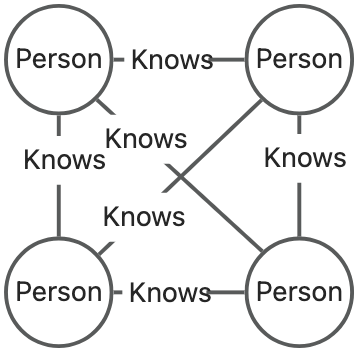
\includegraphics[width=.3\linewidth]{./figures/intro-pattern.png}
    \caption{Pattern graph corresponding to the conditions in the SQL query.}
    \label{fig:intro-pattern}
\end{figure}


Indeed, the conditions specified within this SQL statement collectively establish the structure of a pattern graph.
As shown in Fig.~\ref{fig:intro-pattern}, there are four vertices representing four persons, and these four persons form a complete graph.
Therefore, this SQL query can be expressed as a graph query.
The corresponding expression following the grammar of Cypher \cite{opencypher} is as follows:
\begin{lstlisting}
    MATCH (p1:Person)-[:Knows]-(p2:Person)-[:Knows]-(p3:Person)-[:Knows]-(p4:Person),
        (p1)-[:Knows]-(p3), (p2)-[:Knows]-(p4)
    RETURN p1.id, p2.id, p3.id, p4.id;
\end{lstlisting}
This graph query expression is much more concise and understandable than that in SQL.
It suggests that SQL is not always the optimal choice, and sometimes employing graph queries is more advantageous.
Then, in order to combine the extensive developments made in SQL queries over the years with the benefits of graph queries, it would be helpful for SQL to support both relational and graph queries.

Following this idea, the striking SQL/Property Graph Queries (abbr.~SQL/PGQ) is proposed.
In detail, SQL/PGQ is a part of SQL 2023 and its grammar allows to define and query graphs in SQL/PGQ expressions.
Consequently, some complex relational queries (such as those containing multiple joins) can be represented as relatively simple graph queries.
Specifically, graphs in SQL/PGQ are presented as views, and vertices and edges in the graphs are represented as tables.
It implies that with SQL/PGQ, graph queries and relational queries can be expressed in one statement and optimized together for a better execution plan.
An example of an SQL/PGQ query is provided in Example \ref{example:introduction:sqlpgq}.

\begin{example}
    \label{example:introduction:sqlpgq}
    Suppose three tables, i.e., \textbf{Person, Knows, Department}, are stored in the relational database.
    With SQL/PGQ, a graph view named \textbf{friendship\_graph} is created based on tables \textbf{Person} and \textbf{Knows}.
    Specifically, rows in table \textbf{Person} represent the vertices in the graph while rows in table \textbf{Knows} represent the edges.
    Besides, the department a person belonging to is stored in table \textbf{Person} as a foreign key (i.e., \textit{dept\_id}).

    Suppose we are going to find three persons satisfying: (1) They know each other; (2) Two of them belong to the Department of Computer Science.
    Then, the corresponding SQL/PGQ query is as follows:
    \begin{lstlisting}
        SELECT pn1, pn2, pn3
        FROM Department p, GRAPH_TABLE (friendship_graph
            MATCH (p1:Person)-[:Knows]-(p2:Person)-[:Knows]-(p3:Person),
            (p1)-[:Knows]-(p3)
            COLUMNS (
                p1.name as pn1,
                p1.dept_id as dept1,
                p2.name as pn2,
                p2.dept_id as dept2,
                p3.name as pn3,
                p3.dept_id as dept3)
        ) f
        WHERE dept1 = p.dept_id
        AND dept2 = p.dept_id AND
        AND p.dept_name = 'Computer Science';
    \end{lstlisting}
    According to the first condition, the obtained three persons should form a triangle.
    It is a problem of pattern matching, and such triangles are searched for on \textbf{friendship\_graph}.
    The output of the graph query is a table (named \textbf{f}) with six columns, i.e., pn1, dept1, pn2, dept2, pn3, and dept3, representing the names of the three persons and the identifiers of the departments they belonging to.

    For the second condition, due to the existence of the foreign key, it is efficient to perform natural join between table \textbf{f} and table \textbf{Department} to obtain the ideal results.
    Please note that the outputs of graph queries are still tables, and the outputs can be treated as tables within relational queries.
\end{example}

To support SQL/PGQ queries, it is more reasonable to enhance relational databases with the capability to process graph queries.
The reason is that relational databases have been widely utilized in both academia and industry, and it is costly and impractical to migrate data from relational databases to graph databases.
After the SQL/PGQ query is parsed, relational databases need to optimize the obtained abstract syntax tree (abbr.~AST).
However, since graph queries are allowed in SQL/PGQ queries, the existing relational databases can hardly optimize ASTs with graph operators.
Intuitively, there are some possible solutions, which can be mainly categorized into four types.
The stages of query optimization that these four types of solution are involved in respectively are shown in Fig.~\ref{fig:catagory}.

\begin{figure*}
    \centering
    \begin{subfigure}[b]{0.4\linewidth}
        \centering
        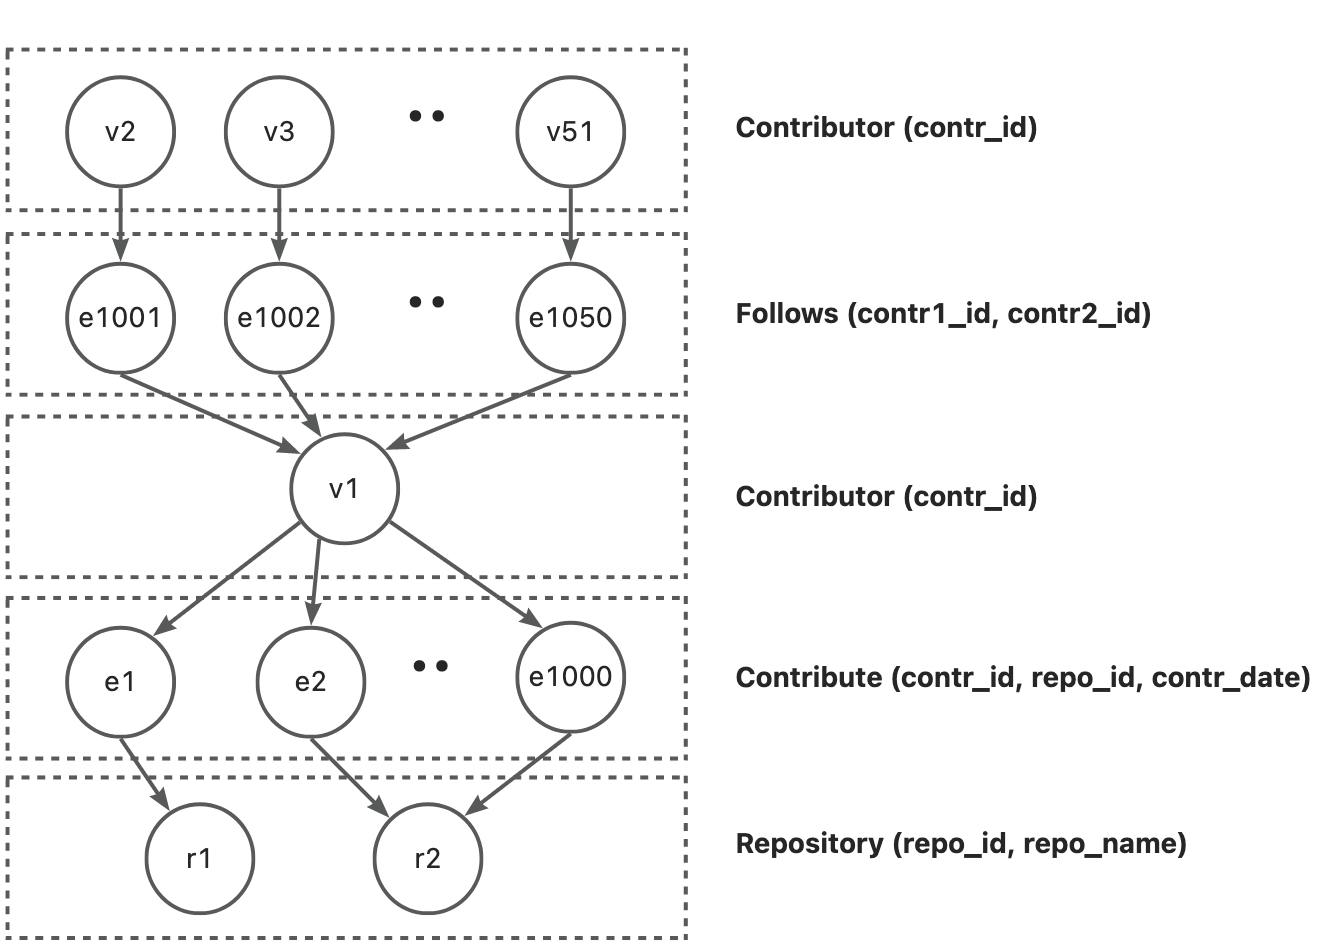
\includegraphics[width=\linewidth]{./figures/intro-order-case.png}
        \caption{Relationship 1.}
        \label{fig:intro-order-case}
    \end{subfigure}
    \begin{subfigure}[b]{0.4\linewidth}
        \centering
        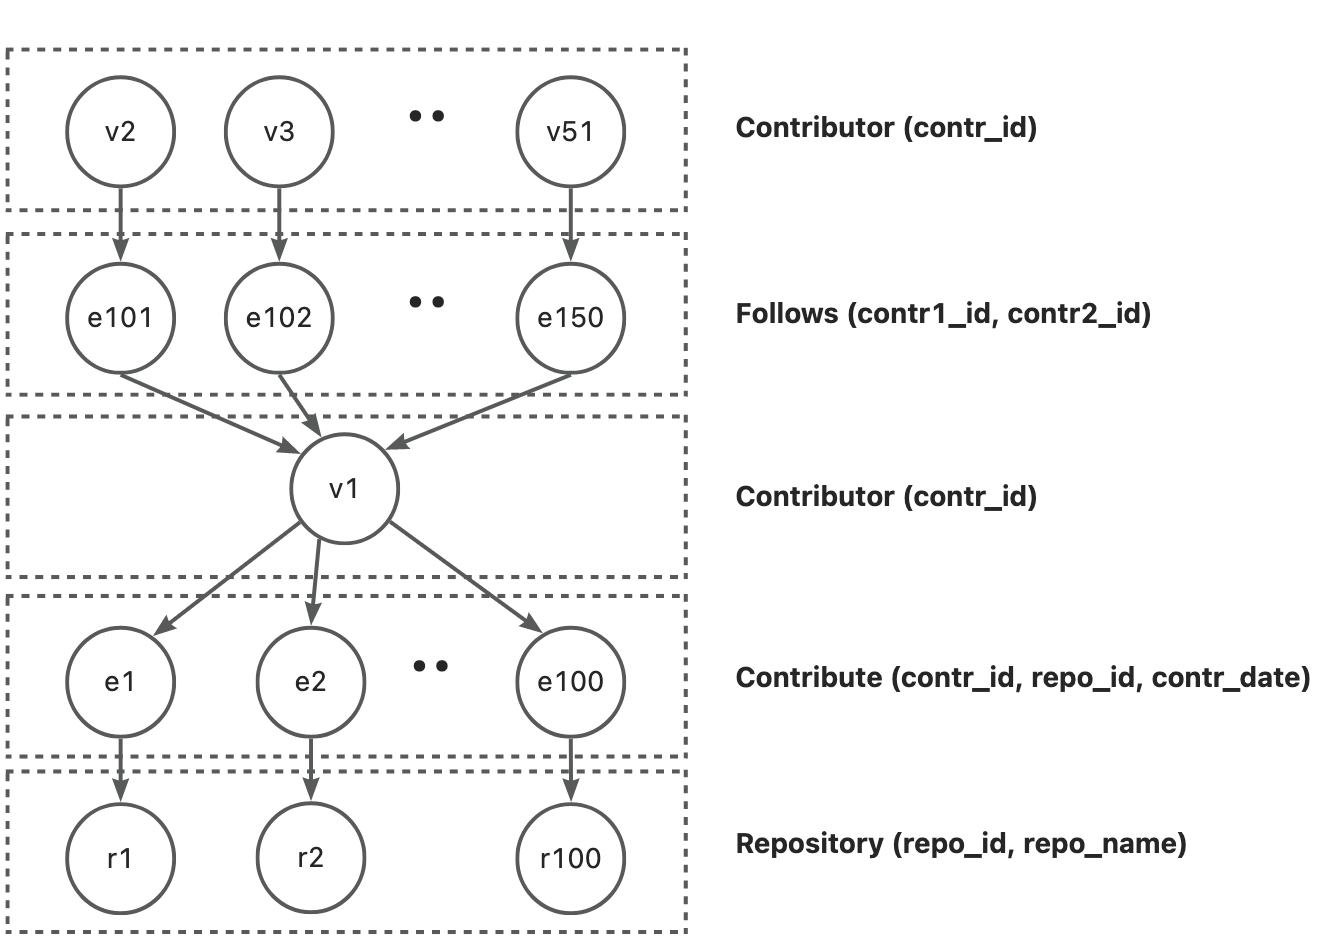
\includegraphics[width=\linewidth]{./figures/intro-order-case-2.png}
        \caption{Relationship 2.}
        \label{fig:intro-order-case2}
    \end{subfigure}
    \caption{Graphs representing the relationships among tuples in different tables. In detail, tuples in Tables \textbf{Contributor} and \textbf{Repository} represent vertices in the graph, while those in Tables \textbf{Follows} and \textbf{Contribute} represent edges.}
    \label{fig:intro-replace-example}
\end{figure*}

\begin{figure*}
    \centering
    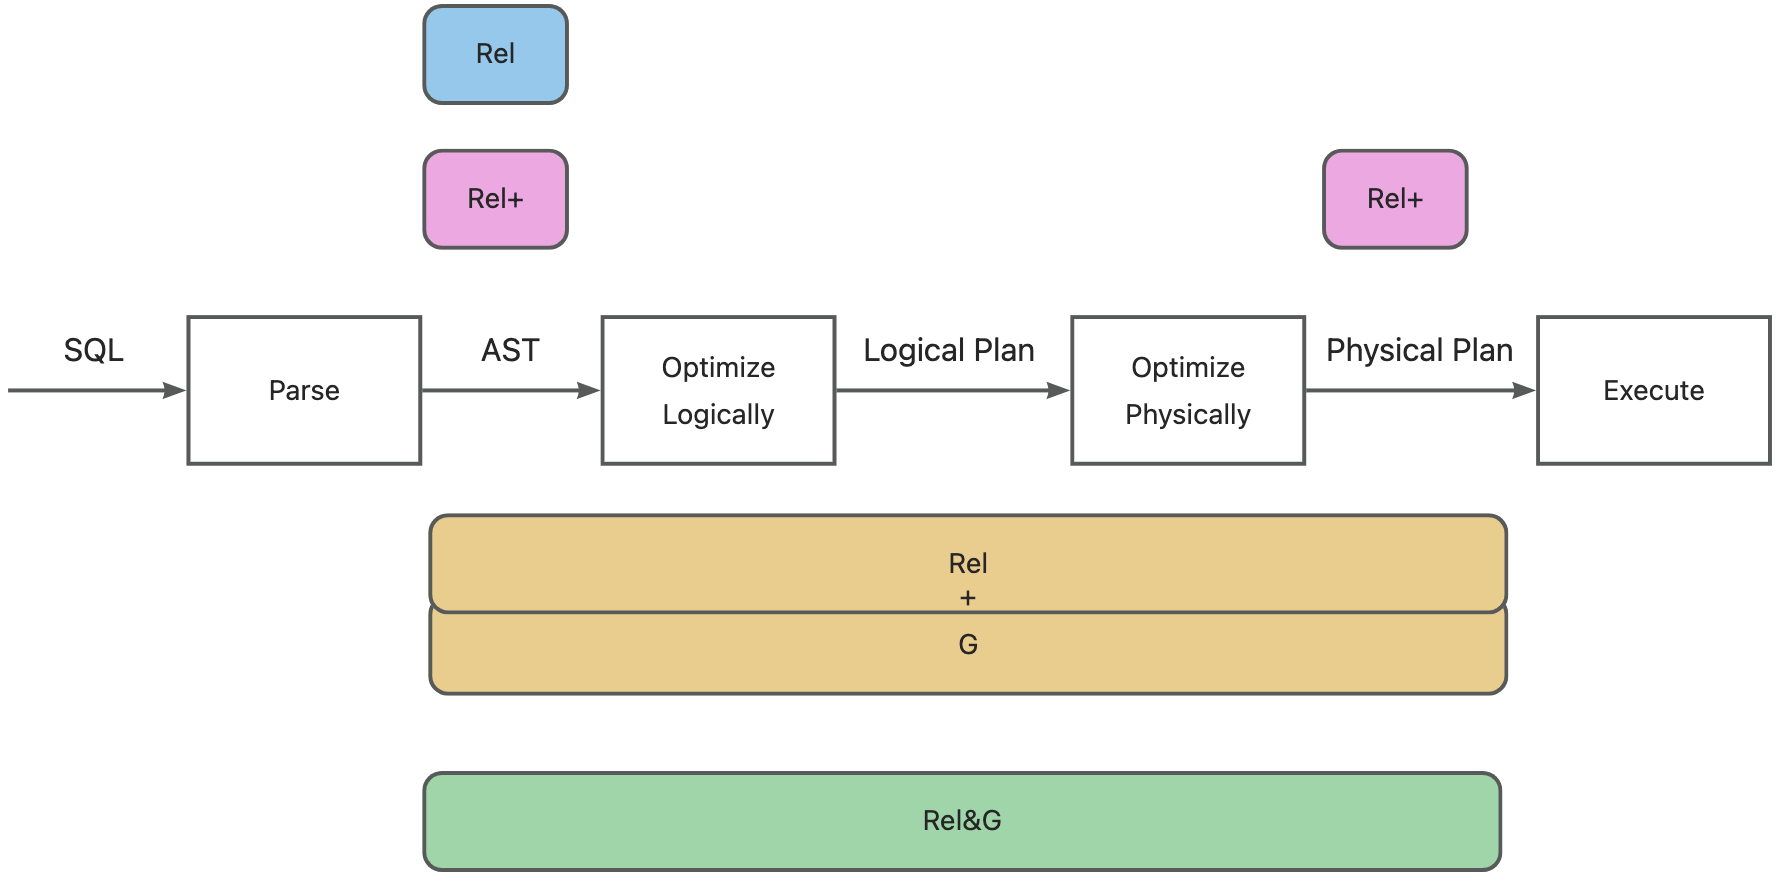
\includegraphics[width=.6\linewidth]{./figures/catagory.png}
    \caption{The stages of query optimization that the four kinds of solutions are involved in.}
    \label{fig:catagory}
\end{figure*}

\textbf{Solution 1 ($Rel$)}.
The most direct solution is to transform graph queries to relational ones, and then optimize the new queries with relational optimizers.
Apache Age \cite{apache-age} and DuckPGQ \cite{DuckPGQ,DuckPGQ-VLDB} are typical examples.
However, methods of this type only take effect in the stage of logical optimization and degrade into relational optimizers.
Therefore, they lose the chance of query optimization from the graph perspective.

\begin{example}
    Given four tables \textbf{Contributor}, \textbf{Follows}, \textbf{Contribute}, and \textbf{Repository} as shown in Fig.~\ref{fig:intro-order-case}, the relationships among their tuples are presented.
    Specifically, edge (v1, e1) means that e1.contr\_id = v1.contr\_id and edge (e1, r1) means that e1.repo\_id = r1.repo\_id.
    Moreover, suppose graph indices have been built on tables \textbf{Follows} and \textbf{Contribute}.
    Then, given a contributor, the followers of the contributor and the repositories the contributor contributes to can be directly retrieved with the indices, respectively.

    Suppose we are going to find the followers of $v1$, and the query is as follows:
    \begin{lstlisting}
        SELECT pid
        FROM GRAPH_TABLE (graph_view
            MATCH (p1:Contributor)-[:Follows]->(p2:Contributor {id: 1})
            COLUMNS (p1.id as pid)
        );
    \end{lstlisting}
    If the graph query is transformed to the corresponding relational query, then the followers of $v1$ can only be found with a join between \textbf{Contributor} and \textbf{Follows}, and another join between the resultant table and \textbf{Contributor}.
    In this process, the graph indices cannot be utilized, and the process is far from efficient.
\end{example}


\textbf{Solution 2 ($Rel^+$)}.
Methods of this type build graph indices on relational databases and introduce new operators to perform graph queries based on the indices.
However, these new operators are applied after the optimal physical plan is obtained with the relational optimizer.
As shown in Fig.~\ref{fig:catagory}, such methods are separately involved in the stages of logical optimization and physical optimization.
It means that the optimizations w.r.t.~graph operators at the logical layer and the physical layer are disjointed.
To be more specific, the cost of new operators introduced in physical optimization are unaware in logical optimization.

The optimizer in GrainDB \cite{graindb} is a representative of type $Rel^+$.
GrainDB builds RID indices on DuckDB \cite{duckdb}, and proposes two new join methods, i.e., sip-join and merge-sip-join.
In detail, sip-join gets adjacent edges of vertices or gets adjacent vertices of edges based on the RID indices, while merge-sip-join obtains the neighbors of vertices.
Since GrainDB follows the grammar of SQL, given a SQL/PGQ query, the query is transformed to the equal relational query first, and then GrainDB optimizes the query with the relational optimizer of DuckDB to obtain the optimal execution plan.
Next, GrainDB replaces some hash-joins in the plan with sip-joins and merge-sip-joins to leverage the graph indices.
It indicates that the cost-based optimization in GrainDB only finds the optimal execution plan before the graph indices are aware.
Therefore, the plan can be suboptimal after replacement.
Moreover, some efficient replacement cannot be applied w.r.t.~the obtained execution plan due to the order of joining tables representing vertices and edges.
An example is shown as follows.

\begin{example}
    Given four tables as shown in Fig.~\ref{fig:intro-order-case}, a SQL/PGQ query is as follows:
    \begin{lstlisting}
        SELECT contr_id, repo_name
        FROM GRAPH_TABLE (graph_view
            MATCH (p2:Contributor)-[f:Follows]->(p1:Contributor {contr_id: 1})-[c:Contribute]->(r:Repository)
            COLUMNS (p2.contr_id as contr_id,
                    r.repo_name as repo_name)
        );
    \end{lstlisting}
    %\begin{lstlisting}
    %    SELECT p2.contr_id, repo_name
    %    FROM Contributor p1, Follows f, Contributor p2, Contribute c, Repository p
    %    WHERE p1.contr_id = 1
    %    AND p1.contr_id = f.contr2_id
    %    AND p2.contr_id = f.contr1_id
    %    AND p1.contr_id = c.contr_id
    %    AND c.repo_id = r.repo_id;
    %\end{lstlisting}
    From the perspective of a relational database (e.g., DuckDB), the best join order can be \textbf{p1$\rightarrow$f$\rightarrow$p2$\rightarrow$c$\rightarrow$r}, since tables \textbf{Follows} and \textbf{Contributor} have much smaller cardinalities than table \textbf{Contribute}.
    Then, by replacing the join operators with getNeighbor, the finally obtained execution plan is \textbf{p1$\xrightarrow{\textit{getNeighbor}}$p2$\xrightarrow{\textit{getNeighbor}}$r}.

    However, as $v_1$ has much fewer neighbors in table \textbf{Repository} than in table \textbf{Contributor}, join order \textbf{p1$\xrightarrow{\textit{getNeighbor}}$r$\xrightarrow{\textit{getNeighbor}}$p2} would be more efficient from the perspective of graph databases.
    Therefore, it suggests that
    replacing relational operators with graph operators after optimization with relational optimizers can miss optimal execution plans.

    Besides, given the relationships among the tuples as shown in Fig.~\ref{fig:intro-order-case2}, the best join order from the perspective of a relational database like DuckDB can be \textbf{p1$\rightarrow$f$\rightarrow$c$\rightarrow$p2$\rightarrow$r}.
    Then, \textbf{p1$\rightarrow$f} and \textbf{c$\rightarrow$p2} cannot be replaced with \textbf{p1$\xrightarrow{\textit{getNeighbor}}$p2} and some efficient execution plans are missing.

    %An example about replace join with getV/getE/getNeighbor,
    %or the example of duckdb, whether to indicate more constraints (due to the unawareness of getNeighbor)
\end{example}


\textbf{Solution 3 ($Rel+G$)}.
According to the grammar of SQL/PGQ, the graph queries usually starts with keyword GRAPH\_TABLE.
Therefore, graph queries can be easily distinguished in SQL/PGQ queries.
Hence, it is possible to optimize graph queries first with graph optimizers, and then optimize the relational query with relational optimizers.
As shown in Fig.~\ref{fig:catagory}, the logical and physical optimization are related, and the cost of graph operators are estimated in the process of optimization.
However, this solution still has limitations, e.g., graph queries and relational queries are optimized separately, and cross-queries optimizations are missing.
An example about this limitation is presented.

\begin{example}
    \label{example:push_down}
    Suppose we are going to find persons that know John and the query expression is as follows:
    \begin{lstlisting}
        SELECT p FROM GRAPH_TABLE (friendship_graph
            MATCH (p1:Person)-[:Knows]-(p2:Person)
            COLUMNS (p1.name as p, p2.name as p2)
        )
        WHERE p2 = 'John';
    \end{lstlisting}
    For $Rel+G$ methods, the graph query is first optimized with a graph optimizer, and the optimized plan finds all pairs of persons that know each other.
    Then, the relational optimizer optimizes the relational query, which finds the persons that know John.
    Please note that the condition ``p2 = 'John''' in the relational query can be pushed down into the graph query, so that the graph query only returns persons that know John.
    The optimized query is as follows.
    \begin{lstlisting}
        SELECT p FROM GRAPH_TABLE (friendship_graph
            MATCH (p1:Person)-[:Knows]-(p2:Person {name: 'John'})
            COLUMNS (p1.name as p)
        );
    \end{lstlisting}
    However, since $Rel+G$ methods optimize relational queries and graph queries separately and do not apply cross-queries optimizations, the condition cannot be pushed down and the optimal execution plan is missed.
\end{example}

In this paper, we propose \textbf{Solution 4 ($Rel\&G$)}, which optimizes the graph queries and relational queries simultaneously with cross-queries optimizations.
Such a solution can fully leverage the advantages of both relational optimizers and graph optimizers.
In detail, we propose a new converged optimization framework of this type for SQL/PGQ.
The framework first generates the converged logical plan consisting of a relational subplan and several graph subplans.
Then, optimization strategies including CBOs and RBOs are applied to optimize inside and crossing subplans.
The contributions of this paper are mainly as follows:

(1) To the best of our knowledge, this is the first optimization framework for SQL/PGQ query optimization.
Property graphs are represented as views in SQL/PGQ, and vertices and edges are associated with tables in the relational databases.
Then, it is crucial to offer a converged query optimizer efficient for SQL/PGQ queries to optimize both relational and graph queries in SQL/PGQ statements.

(2) The framework proposes a new Scan operator named ScanGraphTable to retrieve data from graph tables obtained with graph queries.
The output of ScanGraphTable is a relational table and it bridges the gap between graph subplans and relational subplans.

(3) We prove that graph pattern matching expressed in graph queries of SQL/PGQ can be expressed with graph relational algebra, which confirms that the converged graph relational optimization framework can optimize SQL/PGQ queries and obtain correct results.


% In the framework, we design and implement numerous important operators for graph optimizer, including getV, getE, getNeighbor, and extendIntersect.
% Specifically, the extendIntersect operator is helpful in supporting worst-case optimality.

(4) Theoretical analysis on the complexity of the optimization framework is conducted.
The obtained theorems prove that for graph queries, the join order optimization with a graph optimizer can be exponentially faster than that with a relational optimizer.
It theoretically confirms that relational optimizer is usually not suitable for graph queries, and it is indispensable for the existence of a converged optimization framework.

(5) Extensive experiments are conducted to show the efficiency of the proposed converged query optimization framework.
The experimental results show that the framework can be ?$\times$ faster than the baselines.

The rest of this paper is organized as follows.


The existing methods for optimizing the SPJM queries can be divided into four categories.
The main difference between these methods lies in the approach to handling the matching operator.
Before the details of these methods are introduced, concepts about graph structure and graph matching decomposition are proposed as follows.
}
